\documentclass{article}

\usepackage[normalem]{ulem}
\usepackage{amsthm}
\usepackage{mathtools}
\usepackage{thmtools}
\declaretheoremstyle[headfont=\normalfont]{normalhead}
\usepackage{color}
\usepackage{graphicx}
\usepackage{morefloats}

\usepackage{hyperref}
\hypersetup{
    colorlinks=true,
    linkcolor=blue,
    filecolor=magenta,      
    urlcolor=blue
}

\usepackage{ amssymb }
\usepackage{textcomp}
\usepackage{listings}

\usepackage{url}
\usepackage{float}
\usepackage{biblatex}
\addbibresource{hecke.bib}
\newtheoremstyle{mydef}
{\topsep}{\topsep}%
{}{}%
{\itshape}{}
{\newline}
{%
  \rule{\textwidth}{0.0pt}\\*%
  \thmname{#1}~\thmnumber{#2}\thmnote{\-\ #3}.\\*[-1.5ex]%
  \rule{\textwidth}{0.0pt}}%
  
\begin{document}

\theoremstyle{mydef}
\newtheorem{conjecture}{Conjecture}
\newtheorem{theorem}{Theorem}
\newtheorem{question}{Question}
\newtheorem{remark}{Remark}
\newtheorem{proposal}{Proposal}
\newtheorem{lemma}{Lemma}
\newtheorem{corollary}{Corollary}
\newtheorem{observation}{Observation}
\author{Maksim Kumundzhiev; Bálint Molnár}


\title{Classic CHAID versus Artificial CHAID}
\maketitle
\begin{abstract}
\hskip -.2in
\noindent

Within the last decade it was utilized a lot of research investigations and obtained significant rewards in the field of Artificial Intelligence with emphasizing of Deep Learning area as \href{https://techlurn.org/milestone-achievements-ai-decade.html}{AI insider journal reports}. In the provided list of areas Financial Technology takes pride of place, meaning the importance of continuous research and development has huge impact nowadays. Jointly this work it was investigated and solved welly common FinTech challenge such as "Credit Card Fraud Detection problem". In conjunction it was developed and utilized the robust approach which originates from the random forest method which ingrained by Breiman \cite{Breiman2001} called Neural Forests.  The approach discern by realigning the naive random forests into a neural forests jointly two dedicated ways of training the model. Both approaches inherit classification trees architecture and logic behind. On top of that it was stood a chance to downturn the amount of parameters to incline. The acquired results allowed to emphasise the competitiveness of the developed approach. 
\end{abstract}

\section{Introduction}
Conducting the overview of the classification and the regression machine learning methods we stick around with the one of most popular – a decision tree. 

\section{Related Work}
% Encount previous works which rely on the current topic of the paper.


\section{Decision Trees}
Decision trees are utilized in everyday life decisions what can be invisible from the first point of view. The history of decision trees originates a long time ago and can encount more than 50 years overall of research and development.  
The person who had the major impact of popularisation and expanding the decision trees to the random forest algorithm within his publication is Leo Breiman \cite{Breiman2001}. A decision tree is frequently a generalization of the experts experience, meaning sharing knowledge of a certain process. For instance, before the introduction of scalable machine learning algorithms, the credit scoring task in the banking sector was solved by experts personally. The decision whether to grant a loan was made on the basis of some intuitively (or empirically) derived rules that could be represented as a decision tree. As well it is important to emphasize the following notations:
\begin{itemize}
    \item Root Node: represents the entire sample. 
    \item Splitting: represents the process of dividing a node into sub-nodes. 
    \item Decision Node: once a sub-node splits into further sub-nodes.
    \item Leaf: represents nodes which are not split-able anymore.  
    \item Pruning: represents the process of removing the sub-nodes.
    \item Sub-Tree: represents the subsection of the entire tree.
    \item Parent and Child Node: a node, which is divided into sub-nodes is called a parent node of sub-nodes whereas sub-nodes are the child of a parent node.
\end{itemize}

\section{How to build a Decision Trees}
To propose the best approach to dig around the logic behind building the certain tree it is worth to remember the game "20 Questions" \cite{Stocco2015}. This game allows to make an intuitive reference taking into consideration the goal of the game is to ask such question which will let you narrow down the number of the remaining questions and guess the person. This reasoning corresponds to the concept of information gain based on entropy.
\begin{figure}[h]
    \centering 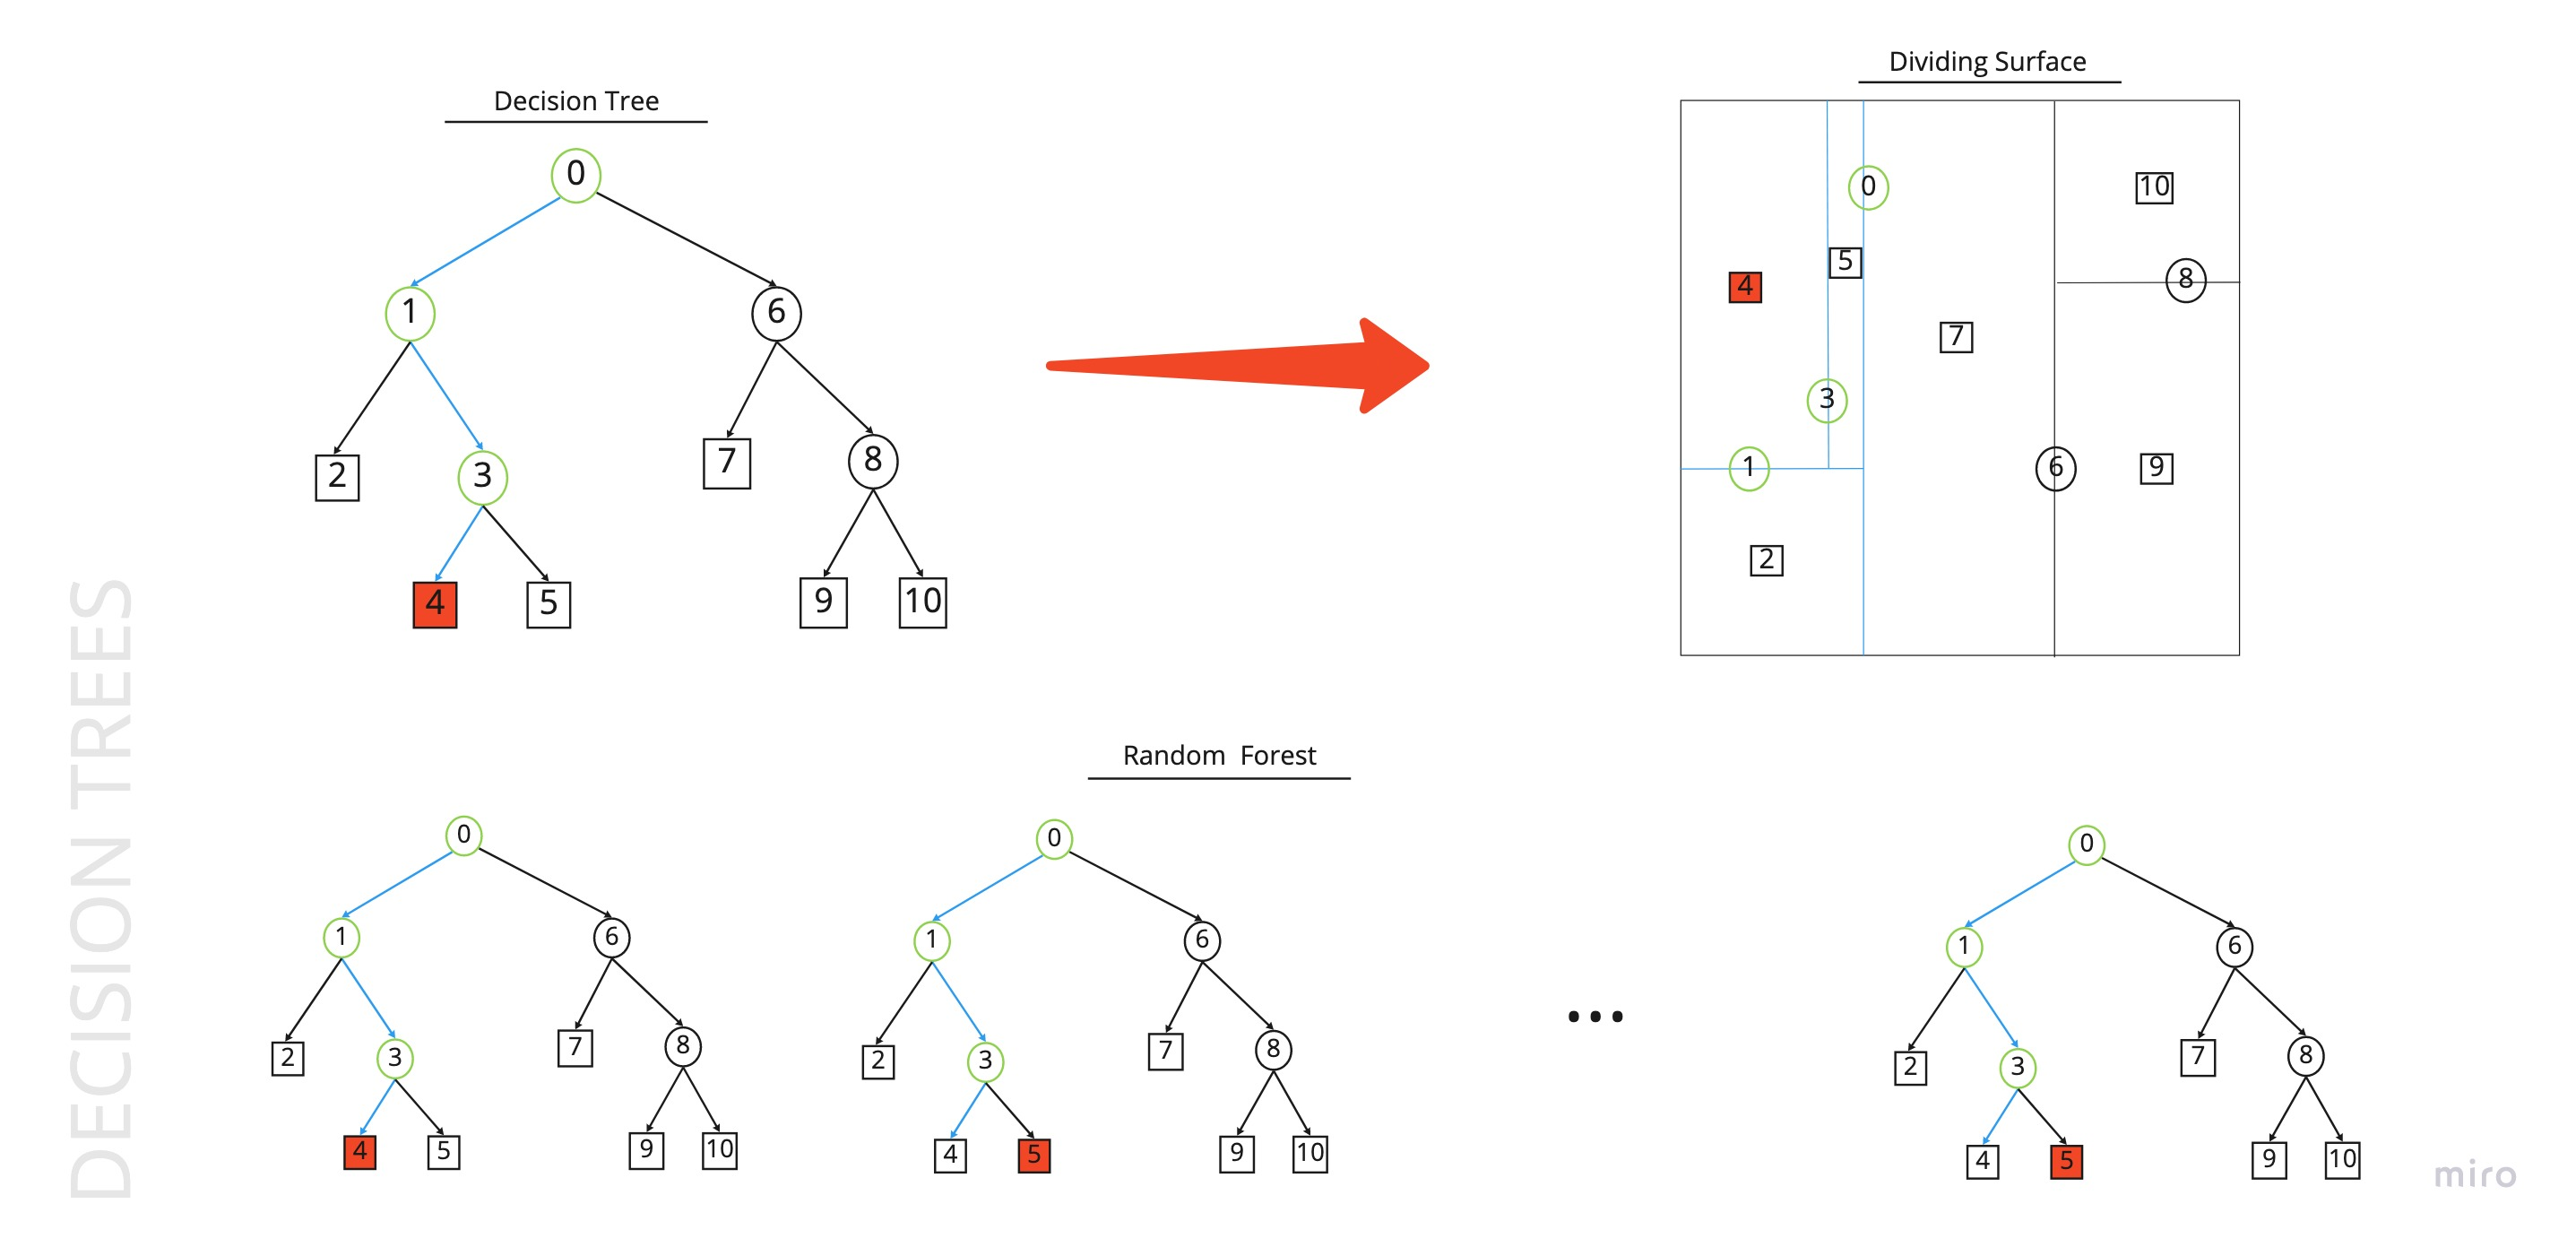
\includegraphics[width=10cm]{images/DTrees.jpg}
    \caption {The high level overview of decision tree and random forest.}
    \label{fig:ct_spine}
\end{figure}


\subsection{Entropy}
The Shannon's entropy \cite{Lotfi2010} is defined for a system with $N$ possible states as follows:
\[ \Large S = -\sum_{i=1}^{N}p_i \log_2{p_i}, \]
where $p_i$ is the probability of finding the system in the $i$-th state. 

It is an important concept used in physics, information theory, as well as in other areas. Entropy can be described as the degree of chaos in the system. The higher the entropy, the less ordered the system and vice versa. This will help us to formalize "effective data splitting", which we alluded to in the context of "20 Questions".

Since entropy is, in fact, the degree of chaos (or uncertainty) in the system, the reduction in entropy is called information gain. Formally, the information gain $IG$ for a split based on the variable $Q$ is defined as: 
\[ \Large IG(Q) = S_O - \sum_{i=1}^{q}\frac{N_i}{N}S_i, \]
where $q$ is the number of groups after split, $N_i$ is the number of the objects from the sample in which $Q$ is equal ti the $i$-th value. 

\subsection{Gini Index}
In simplified terms Gini Index stands for maximization of the number of pairs of objects of the same class that are in the same subtree (not to be confused with the Gini index) and can be derived as: 
\[ G = 1 - \sum\limits_k (p_k)^2 \]

\subsection{Tree-building Algorithms}
Decision trees use multiple algorithms to decide to split a node into two or more sub-nodes. The creation of sub-nodes increases the homogeneity of resultant sub-nodes. In other words, we can say that the purity of the node increases with respect to the target variable. The decision tree splits the nodes on all available variables and then selects the split which results in most homogeneous sub-nodes. There are various algorithms to utilize but we will focus on two main ones.  
\subsubsection{CART}
%TBD
The representation of Classification And Regression Tree is a binary tree. Each root node represents a single input variable $x$ and a split point on that variable (assuming the variable is numeric). The leaf nodes of the tree contain an output variable $y$ which is used to make a prediction.

Creating a CART model involves selecting input variables and split points on those variables until a suitable tree is constructed.

The selection of which input variable to use and the specific split or cut-point is chosen using a greedy algorithm to minimize a cost function. Tree construction ends using a predefined stopping criterion, such as a minimum number of training instances assigned to each leaf node of the tree.

\subsubsection{CHAID}
%TBD
Chi-Squared Automatic Interaction Detection was proposed by Kass \cite{Lewis-Beck2012} in 1980. As is evident from the name of this algorithm, it is based on the chi-square statistic. A Chi-square test yields a probability value as a result lying anywhere between 0 and 1. A chi-square value closer to 0 indicates that there is a significant difference between the two classes which are being compared. Similarly, a value closer to 1 indicates that there is not any significant difference between the 2 classes. 



\section{Neural Networks}
Typically, neurons are kind of information messengers who make use of electrical and chemical gusts to transfer information across all brain moreover between brain and rest of the nervous system.

\subsection{Biological neuron}
A neuron is a component that makes up the entire human nervous system. Almost all neurons are structured roughly the same. So, a neuron has a neuron nucleus, which is also called the neuron body. An electrical charge is accumulated in the body of a neuron. From the body of the neuron there are many processes: there are small processes and large processes. The little outgrowths are so called dendrites. Through these processes, a signal from other neurons comes to our neuron. There is a large scion. This process is called an axon. A neuron transmits a signal to other neurons along the axon. The place where the axon of another neuron connects to the dendrites of our neuron is called a "synapse". The synapse is where the dendrite and axon meet. A synapse can be strong or it can be weak. If the synapse is strong, then the signal that is transmitted along the axon of the neuron will almost completely go to our neuron. If the synapse is weak, then practically no charge will cross from the axon of another neuron to our neuron. The synapse can change over time. Depending on the circumstances, the synapse can get stronger or it can get weaker. It is with the synapse tuning that the training of the biological neural network and, accordingly, the human nervous system is connected.

Considered visualization of the described above processes is as follows:
\begin{figure}[h]
    \centering 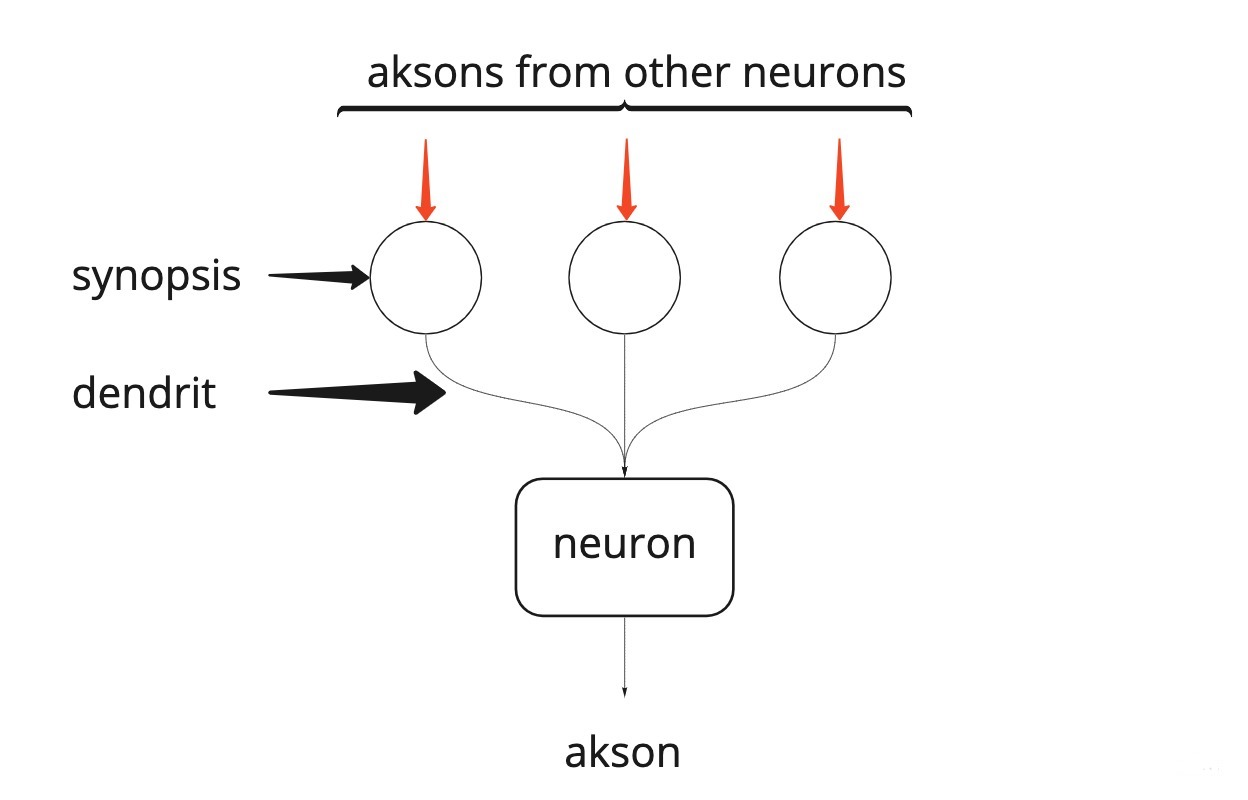
\includegraphics[width=8cm]{images/biological_neuron.jpg}
    \caption {Biological model of neuron.}
\end{figure}    

\subsection{Mathematical model of neuron}
Initially for simplicity we will represent neuron mathematical model graphically. It should be taken into consideration, the red characters denote tune parameters of the neuron.     
\begin{figure}[h]
    \centering 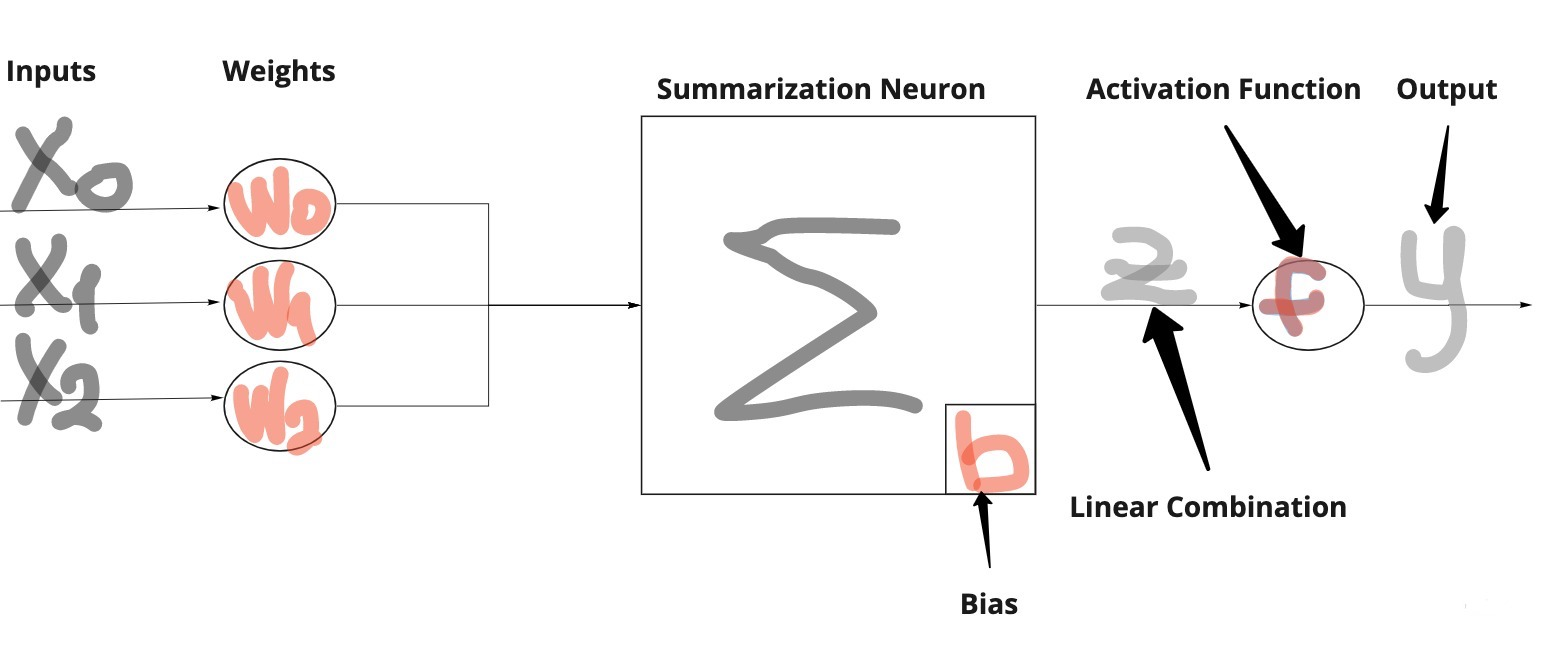
\includegraphics[width=8cm]{images/neuron_math_model.jpg}
    \caption {Mathematical model of neuron.}
\end{figure} 

In the mathematical model of the neuron, the body of the neuron, where the input signals accumulates, is denoted by a summarizing neuron. In addition, the biological neuron also has axons and dendrites, which get the inputs and send the outputs. Accordingly, in our mathematical model of the neuron, we will add inputs and outputs to the summarizing neuron. It's also worth keep in mind the biological neuron applies some actions with the signals that come into it, namely, it accumulates charge until it reaches some point and only after that forwards it further. This is what we will do in the mathematical model of the neuron using the activation functions.

Afterwards, let us mathematically define model of neuron as:
\begin{align*}
y = f(z) = f(w_0 \cdot x_0+w_1 \cdot x_1+w_2 \cdot x_2+b) = f(\sum\limits_{i=0}^{N-1} w_i \cdot x_i+b) = f(\langle w, x \rangle + b)
\end{align*}
Where: $x_0, x_1, x_2$: inputs, $w_0, w_1, w_2$: weights,  $b$: some bias for increasing non-linearity, $f(z)$: some activation function. 

Inputs can be either single number or vector of numbers. As for weights, we mainly should remember they are tuned parameters. Moreover it should be considered 2 potential situations to manage with. The first one is initialization of the weights. Here we have multiple options whereas we literally can define them either randomly or apply special initialisation techniques such as "He" initialization or "Xavier" initialization and others. The second situation we should be aware of is to somehow change the weights during model fitting, meaning weights should be changed in iterative manner from epoch to epoch. To do this we will apply backpropagation algorithm. Concerning the bias, which is like a weights, meaning tuned parameter, we can consider it allows to shift the activation function by adding a constant to the input of neuron. Hence, the last but not least component is activation function. In simplified terms, activation function is used to determine the output of neuron in a manner: "yes" or "no". It maps the resulting values in range between 0 to 1 or -1 to 1.            

To conclude, from the code base perspective one neuron functionality can be defined as:
\begin{lstlisting}
def _activation_function(weighted_sum):
  """step function is used as an example"""
  return 1 if weighted_sum > 0 else 0

def _neuron(inputs, weights, bias):
  weighted_sum = 0
  for input_vector, weight_vector, bias_vector in zip(inputs, weights, bias):
    particular_sum = (input_vector * weight_vector) + bias_vector
    weighted_sum += particular_sum
    output = _activation_function(weighted_sum)
  return output
\end{lstlisting}

      
\section{Activation function}
There is a significant number of various activation functions. Let us assume the very basic one named "step function" and figure out from general point of view how it works in both mathematical and geometrical conditions.   
The "step function" defined as:
\begin{align*}
f(x) = \begin{cases} 0, & \mbox{if } x\mbox{ <= 0} \\ 1, & \mbox{if } x\mbox{ > 0} \end{cases}
\end{align*}

The function has 2 strongly distinguished values: "0" and "1". The "spot" where the function changes it's value from "0" to "1" is named as dividing surface. Hence, the dividing surface "spot" is where the argument of activation function is equal "0".

\begin{figure}[h]
    \centering 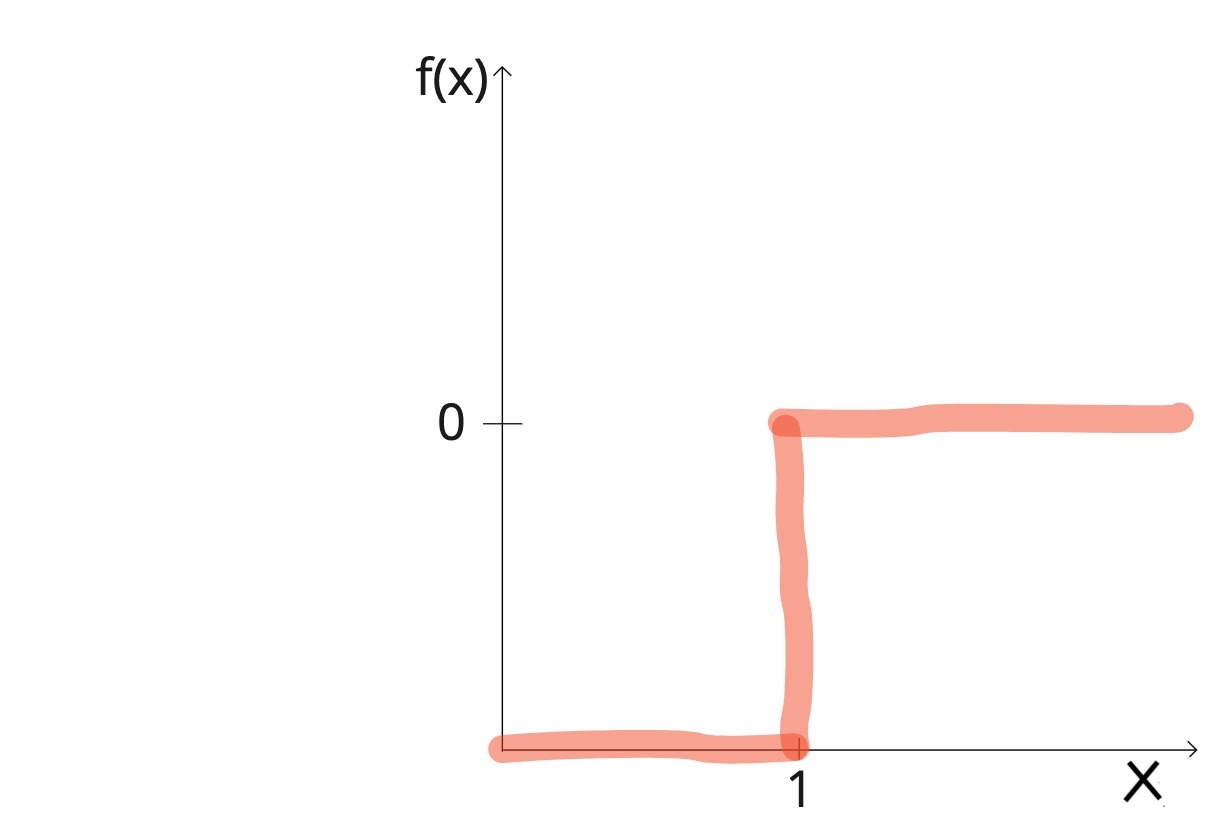
\includegraphics[width=8cm]{images/step_function.jpg}
    \caption {Step function geometrical representation.}
\end{figure}

The geometrical representation of step function can be derived as following. Assume there is the neuron formula:
\begin{align*}
y = f(\langle w, x \rangle + b)
\end{align*}

The neuron does some linear operation, which is denoted by 2 parameters:
\begin{itemize}
    \item $w$: vector of weights
    \item $b$: bias
\end{itemize}
Accordingly, the dividing surface is defined by following equitation which denotes equitation of straight line:
\begin{align*}
\langle w, x \rangle + b = 0
\end{align*}

\begin{figure}[h]
    \centering 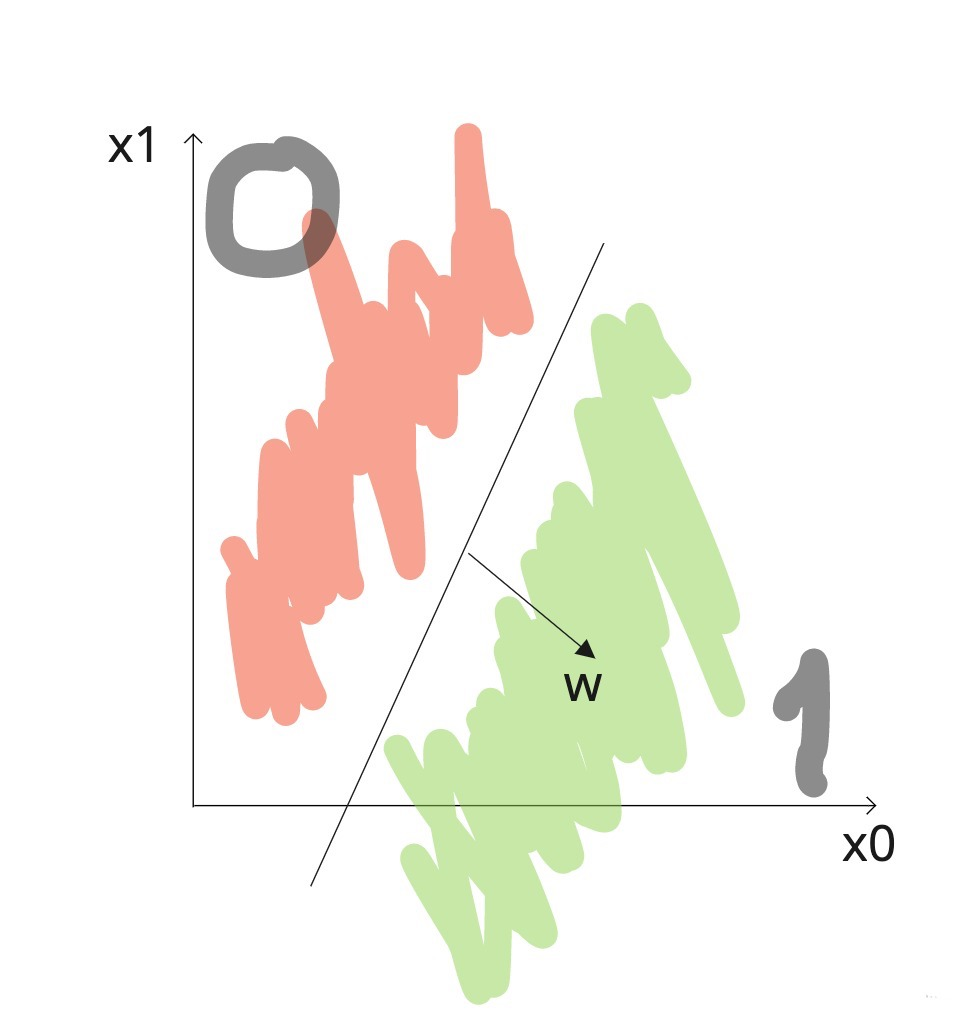
\includegraphics[width=8cm]{images/dividing_surface.jpg}
    \caption {Dividing surface geometrical representation.}
\end{figure}

From the one side the value of step function is equal "1" and from the other "0". The activation function is equal "1" that side of dividing surface where the vector "w" point out.

As for code base representation, step function can be defined as:
\begin{lstlisting}
def _step_function(weighted_sum):
  return 1 if weighted_sum >= 0 else 0
\end{lstlisting}
   
As it was mentioned earlier, step function is not the only one activation function. There is for instance "sigmoid" activation function which unlike step function does not have discontinuity point at zero. 

The sigmoid activation function formed as:
\begin{align*}
\sigma(x) = \dfrac{1}{1+e^x}
\end{align*}

\[ \sigma(x) = \begin{cases} 1, & \mbox{if } x\mbox{$\xrightarrow{} + \infty$} \\ 0, & \mbox{if } x\mbox{$\xrightarrow{} - \infty$} \end{cases} \]

The rectified linear activation function for short is a piece-wise linear function which outputs input directly if it is positive otherwise outputs zero. It has become the default activation function for many types of neural networks because a model that uses it is easier to train and often achieves better performance.

\begin{figure}[h]
    \centering 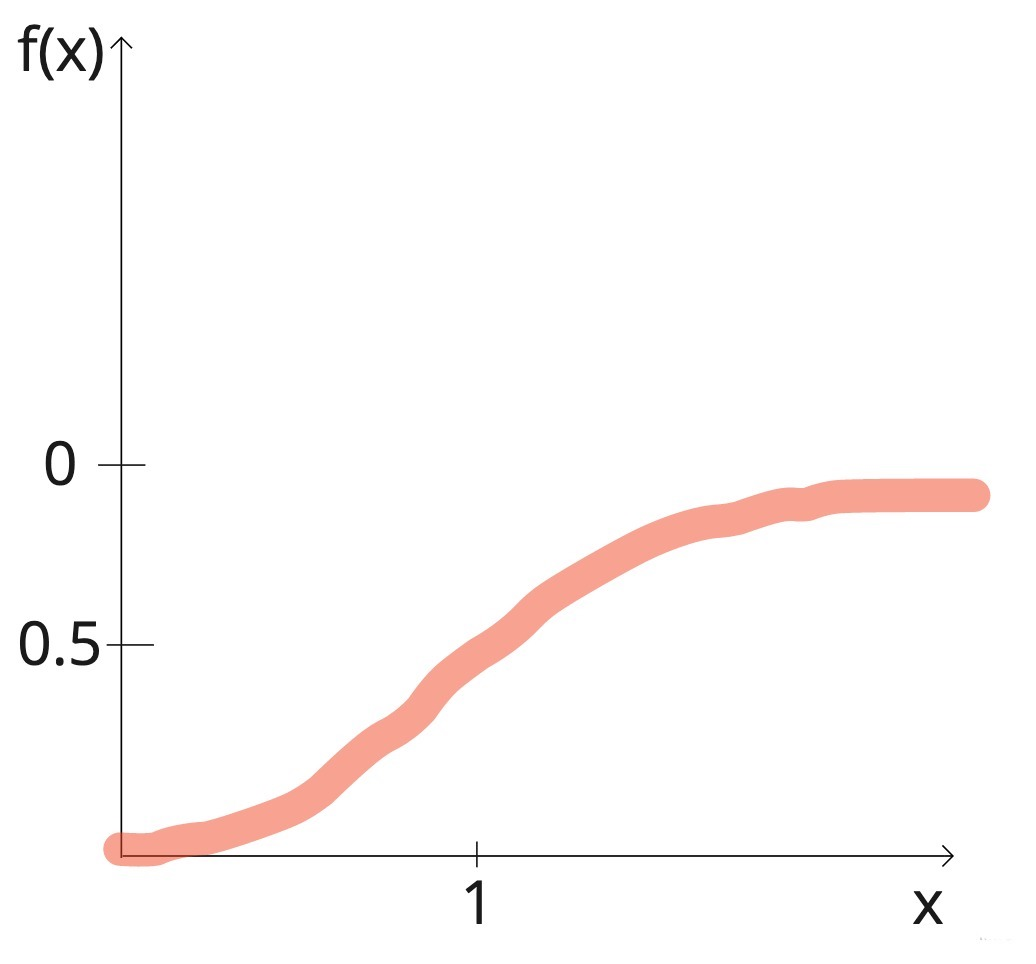
\includegraphics[width=8cm]{images/sigmoid_function.jpg}
    \caption {Sigmoid activation function.}
\end{figure}

\section{From neuron to neural network}
So far we have discussed the properties and functional of a single neuron, which as a result outcomes a linear divide surface in geometrical terms. Meaning when we will concatenate the multiple neurons in some architecture we may achieve some nonlinear divide surfaces.
\begin{figure}[h]
    \centering 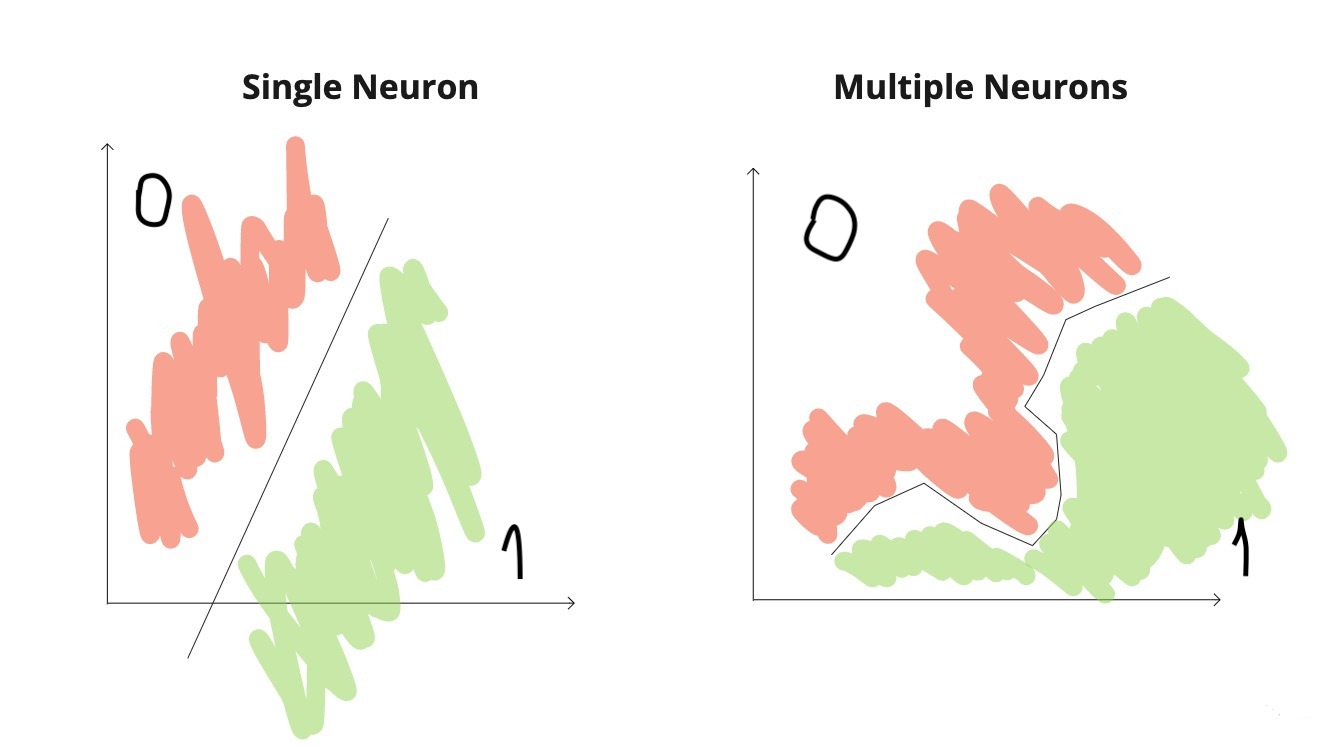
\includegraphics[width=7cm]{images/neuron_to_neural_net.jpg}
    \caption {Single neuron surface vs multiple neurons surface.}
\end{figure}

Now the question is how do we get the nonlinear dividing surface. Let us figure it out.
For simplicity define 3 neurons with linear activation function:
\begin{figure}[h]
    \centering 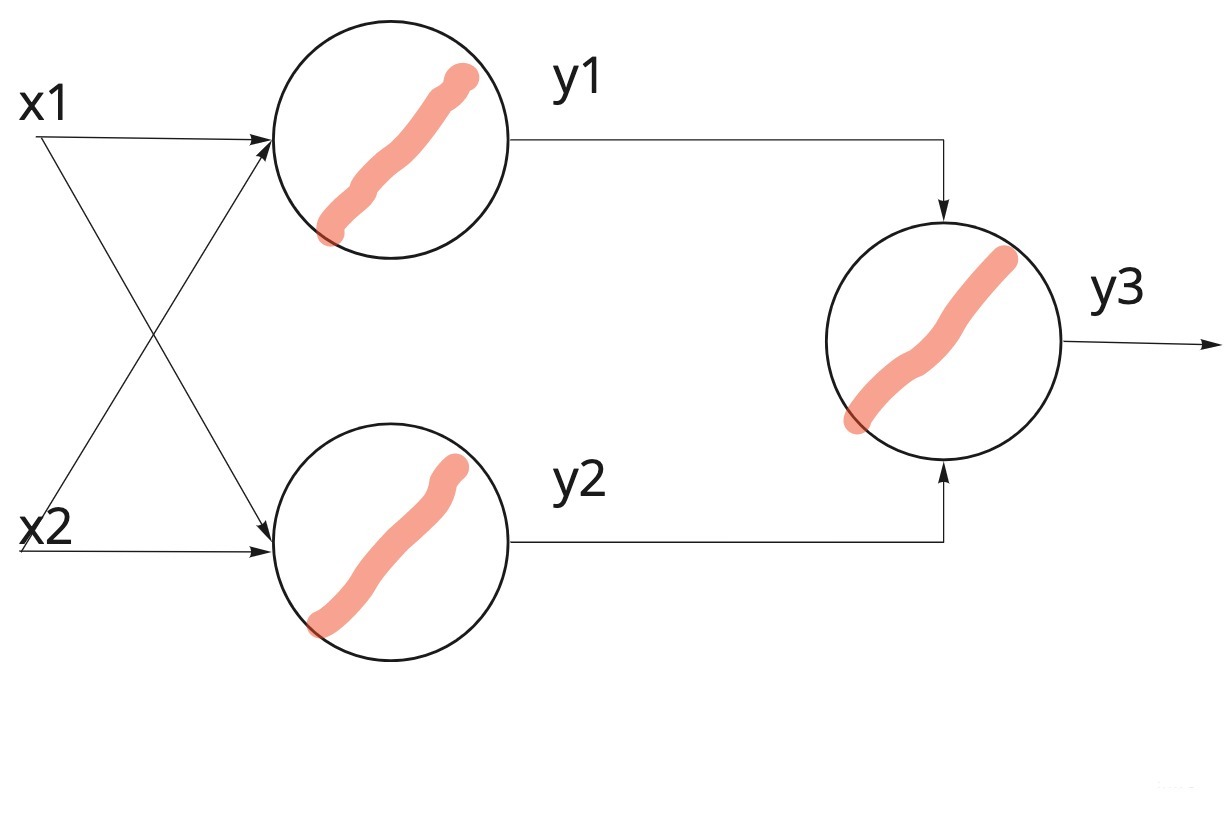
\includegraphics[width=8cm]{images/3_neurons_net.jpg}
    \caption {Neural net with linear activation function.}
\end{figure}
The results of performing the net can be considered as:
\[ y_3 = f(w_2^3 \cdot y_2+w_1^3 \cdot y_1+b^3) = \]
By the reason $f$ is simple linear function, equation can be derived as:
\[ = w_2^3 \cdot y_2+w_1^3 \cdot y_1+b^3 = \] 
\[ = w_2^3 \cdot f(w_2^1\cdot x_1+w_2^2 \cdot x_2+b^2) + w_1^3 \cdot f(w_1^1 \cdot x_1+w_1^2 \cdot x_2+b^1) + b^3 = \]   
\[ = w_2^3 \cdot w_2^1 \cdot x_1+w_2^3 \cdot w_2^2 \cdot x_2+b^2 + w_1^3 \cdot w_1^1 \cdot x_1+w_1^3 \cdot w_1^2 \cdot x_2+b^1+b^3 = \]
\[ = x_1[w_2^3 \cdot w_1^2 + w_1^3 \cdot w_1^1] + x_2[w_2^3 \cdot w_2^2 + w_1^3 \cdot w_2^1] + [w_2^3 \cdot b^2+w_1^3 \cdot b^1+b^3] = \]
\[ =  x_1\cdot \tilde{w_1} + x_2\cdot \tilde{w_2} + \tilde{b} \]
Meaning the obtained result is just linear combination of inputs into the neural net. 

\subsection{Neural network starter kit}
Once we had familiarized ourselves with basic concept of neuron and activation function, we may stand a chance to solve some real problem. But still we need figure few more lacking basic components out.
We can be aware of the uniform starter kit for any neural network can be defined as:
\begin{itemize}
    \item neural net architecture, meaning which parts the net will consist of, how the parts will be connected, how neurons will be defined etc.
    \item neural net optimization function, meaning approaching which optimization algorithm the value of loss function (performance of neural net) could be increased. It worth to keep in mind the optimization process requires a loss function to calculate the model error.
    \item neural net loss function, meaning how the net performs. Moreover, the less loss function value is the better performance of the net is.
    \item neural net metrics, meaning how the net performs. It is similar to loss function, but considered as secondary and optional metric. They does not have impact on the neural net fitting process, however could bring out useful insights.    
\end{itemize}


\section{How neural networks learn?}
It was already discussed trivial neural net architecture consisting of neuron mathematically representation and premise of activation function. As for now let us review clause by clause the rest components which are the driven pieces for nets learning process.

\subsection{Optimization function}
Optimization of neural net is the key component in terms of finding latent patterns in input data. The optimization of the net should be considered as the on-the-spot training. There are variety optimization algorithms but the pillar algorithm in the list is gradient descent.
The brief list of optimization algorithms:
\begin{enumerate}
    \item Gradient Descent
    \item Stochastic Gradient Descent
    \item Mini-Batch Gradient Descent
    \item Nesterov Accelerated Gradient
    \item Momentum
    \item Adagrad
    \item RMSProp
\end{enumerate}
Let us discuss how the optimization works under the hood proceeding with the most demonstrative algorithm -- gradient descent.

\subsection{Gradient descent}
Previously we took into consideration the neural net has 2 main tuned parameters: "weights" and "bias".

Let us concern we have a some function which is defined by some levels lines. The function has 2 minimums, which are denoted by the red dots.  It worth to understand by distancing from the minimums the function value increases. 
So far, we have a neural net with some parameters (weights and biases) which performs some value of loss function. As we remember out main task is to decrease the value of loss function. Hence, the question is how to do that.

\begin{figure}[h]
    \centering 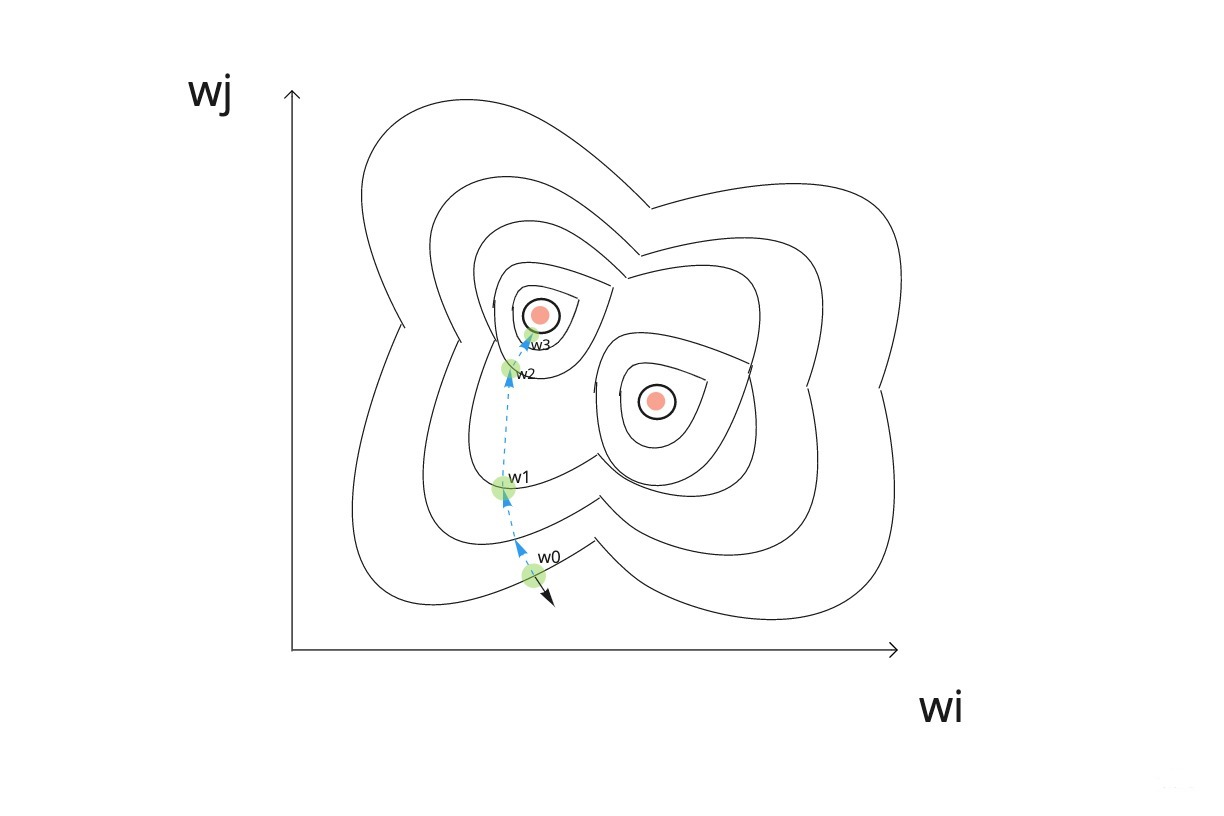
\includegraphics[width=7cm]{images/gradient_descent.jpg}
    \caption {Gradient descent visualization.}
\end{figure}

So, the very first provision in the vector of function surface will be defined by $w_0$, where $w_0$ denotes vector of all weights and biases of the net and can be represented as: 

\[ w_0 = [w_1^1, w_1^2,...,w_1^n, w_2^1,...,w_2^n,...,w_n^n, b1^1, b1^2,...,b1^n, b2^1,...,b2^n,...,b_n^n] \]

Accordingly, we need take derivative (meaning gradient, which is vector consisting of derivatives per each coordinate of the function) of the loss function of our vector. It can be represented as:
\[ \delta{f} = [\frac{\partial{f}}{\partial{w_0}}, \frac{\partial{f}}{\partial{w_1}}, ... ,\frac{\partial{f}}{\partial{w_n}} ] \]
As the result, we have calculated the gradient of loss function at the point ($w_0$) where we currently located. The gradient of loss function points out at the direction of greater loss function growth. But, oppositely, we on demand of lower loss function growth, meaning we need to make an opposite step of calculated gradient descent. It can be considered as:
\begin{align*}
w_1 = w_0 - \alpha \cdot \delta{f(w_0)}
\end{align*}
Let us take a closer look at the formula above:
\begin{itemize}
    \item $w_0$: the initial vector of weights and biases of neural net
    \item $\alpha$: parameter for regulating the "speed" of training the neural net. In other words it affects the size of gradient step 
    \item $\delta{f(w_0)}$: calculated gradient of loss function at the $w_0$ point 
\end{itemize}
The gradient descent of loss function will be calculated until it will not converge some "preciseness" within predefined "fallacy".


From the code base perspective using PyTorch framework, the algorithm considered as:
\begin{lstlisting}
import torch
 x = torch.tensor([[1,2,3,4],[5,6,7,8],[9,10,11,12]],                requires_grad=True) 
function =  10*(x**2).sum()
function.backward()
print(x.grad, '<- gradient')
\end{lstlisting}

\section{How evaluate neural network performance?}
In the terms of an optimization algorithms, function aim to evaluate a distinctive solution (meaning a set of weights) which cite to as objective function. Depending we may search for either to maximize or minimize the objective function. meaning the highest or lowest score respectively.
\subsection{Loss function}
Characteristically neural networks we keen to minimize the error. There are many functions that could be potentially used to estimate error of set of weights in a neural network. Below we consider few popular loss functions.

\subsubsection{Mean Squared Error (MSE)}
Mean Squared Error is the average of the squared error that is used as the loss function for least squares regression. To streamline, MSE is the sum,over all the data points of the square of the difference between the predicted and actual target variables divided by the number of data points.
\begin{align*}
MSE = \frac{{1}}{n} \sum_{i}^{n} (y_i - \widehat{y_i})^2
\end{align*}
where $y$ is the desired Neural Network output, and $\widehat{y_i}$ is the neural network output.

As well it can be programmed as follows:
\begin{lstlisting}
# calculate mean squared error
def mean_squared_error(actual, predicted):
	sum_square_error = 0.0
	for i in range(len(actual)):
		sum_square_error += (actual[i] - predicted[i])**2.0
	mean_square_error = 1.0 / len(actual) * sum_square_error
	return mean_square_error
\end{lstlisting}

\subsubsection{Cross-Entropy}
Cross-entropy loss, or log loss \footnote{https://ml-cheatsheet.readthedocs.io/en/latest/loss_functions.html#cross-entropy}, measures the performance of a classification model whose output is a probability value between 0 and 1. Cross-entropy loss increases as the predicted probability diverges from the actual label.
In binary classification, where the number of classes M equals 2 cross-entropy can be calculated as:
\begin{align*}
Cross-Entropy = -{(y\log(p) + (1 - y)\log(1 - p))}
\end{align*}
And if $M > 2$ meaning we work out multi-classification problem we calculate a separate loss for each class label per observation and sum the result as:
\begin{align*}
Cross-Entropy = -\sum_{c=1}^My_{o,c}\log(p_{o,c})
\end{align*}

As for codebase trivial implementaion it can be formed as:  
\begin{lstlisting}
def cross_entropy(yHat, y):
    if y == 1:
      return -log(yHat)
    else:
      return -log(1 - yHat)
\end{lstlisting}

\section{From Decision Trees to Neural Forest}
%TBD
Consider the $m$-th tree estimate $t(\cdot, \Theta_m, D)$ of the forest, seen as a neural network estimate. Conditional on $\Theta_m$ and $D_n$, the architecture of this network is fixed, and so are the weights and offsets of the three layers. A natural idea is then to keep the structure of the network intact and let the parameters vary in a subsequent network training procedure with backpropagation training. In other words, once the connections between the neurons have been designed by the tree-to-network mapping, we could then learn even better network parameters by minimizing some empirical mean squared error for this network over the sample $D_n$. This additional training can potentially improve the predictions of the original random forest, and we will see more about this later in the experiments.
\begin{figure}[h]
    \centering 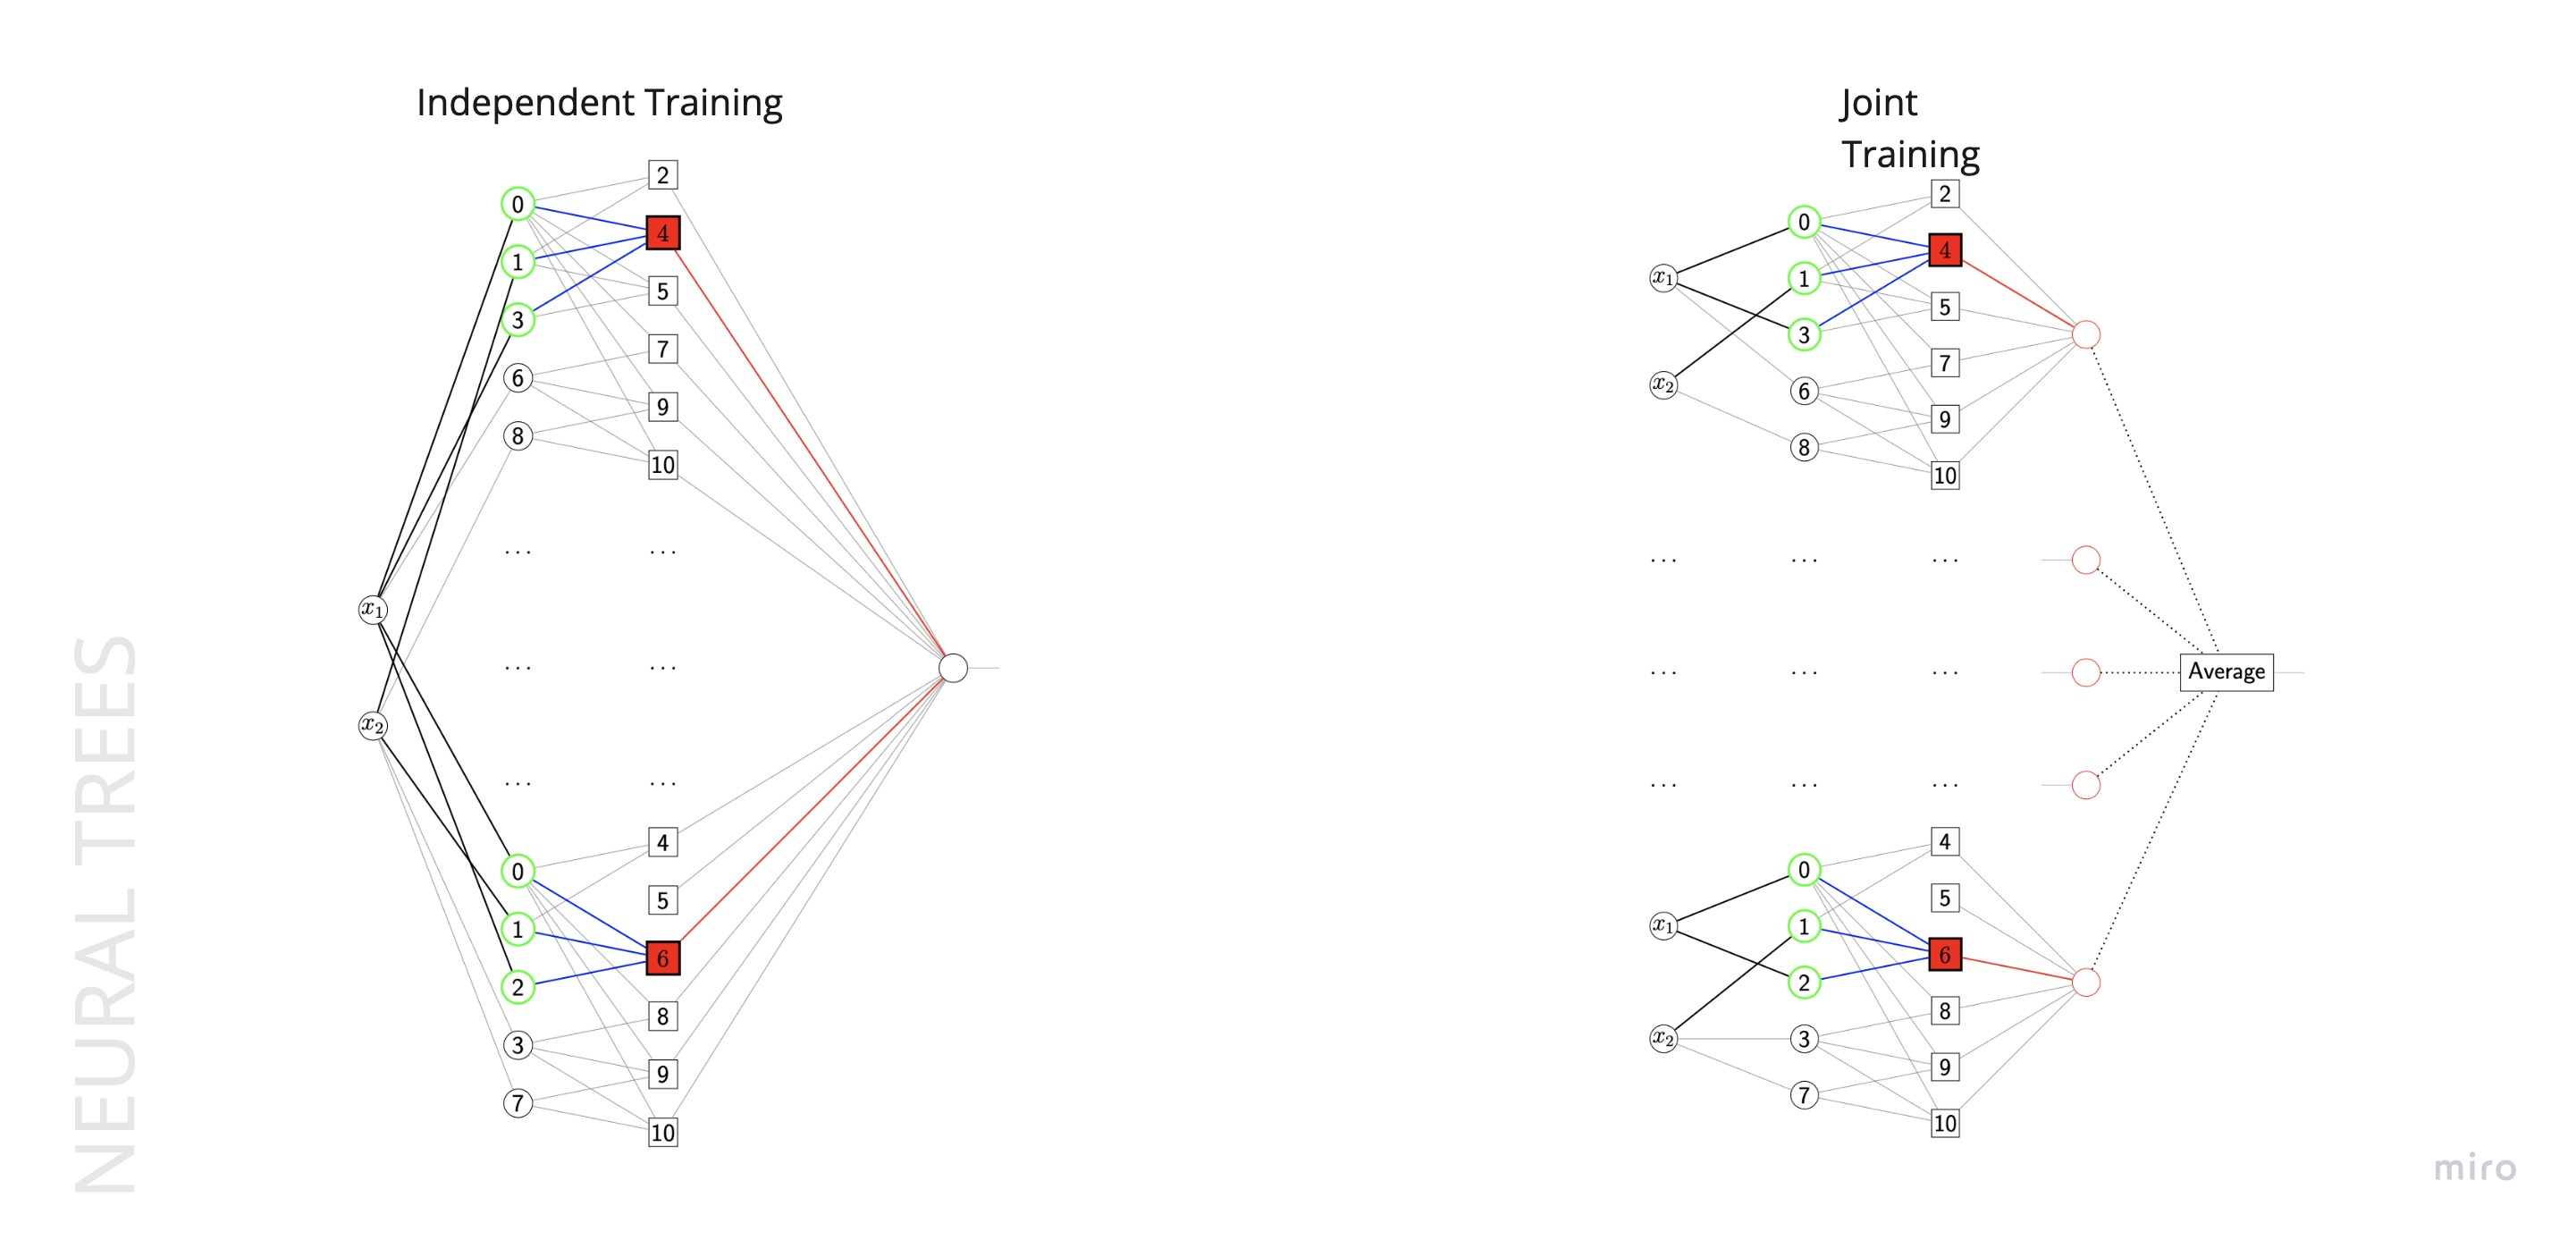
\includegraphics[width=10cm]{images/NeuralTrees.jpg}
    \caption {The high level overview of neural forest.}
    \label{fig:ct_spine}
\end{figure}

To allow for training based on gradient backpropagation, the activation functions must be differential. A natural idea is to replace the original activation function:
\[ \tau(\upsilon)= \dots  \]
%TBD

\subsection{Independent Training}
%TBD
The parameters of each tree-type network are fitted network by network, independently of each other.

\subsection{Joint Training}
%TBD
In this approach, the individual tree networks are first concatenated into one single “big” network. The parameters of the resulting “big” network are then fitted jointly in one optimization procedure over the whole network.

\section{Dataset}
The proposed data was adopted from the Kaggle \href{https://www.kaggle.com/mlg-ulb/creditcardfraud}{"Credit Card Fraud Detection" competition}. The datasets contains transactions made by credit cards in September 2013 by European cardholders. 
This dataset presents transactions that occurred in two days, where we have 492 frauds out of 284,807 transactions. The dataset is highly unbalanced, the positive class (frauds) account for 0.172\% of all transactions.

\begin{figure}[h]
    \centering 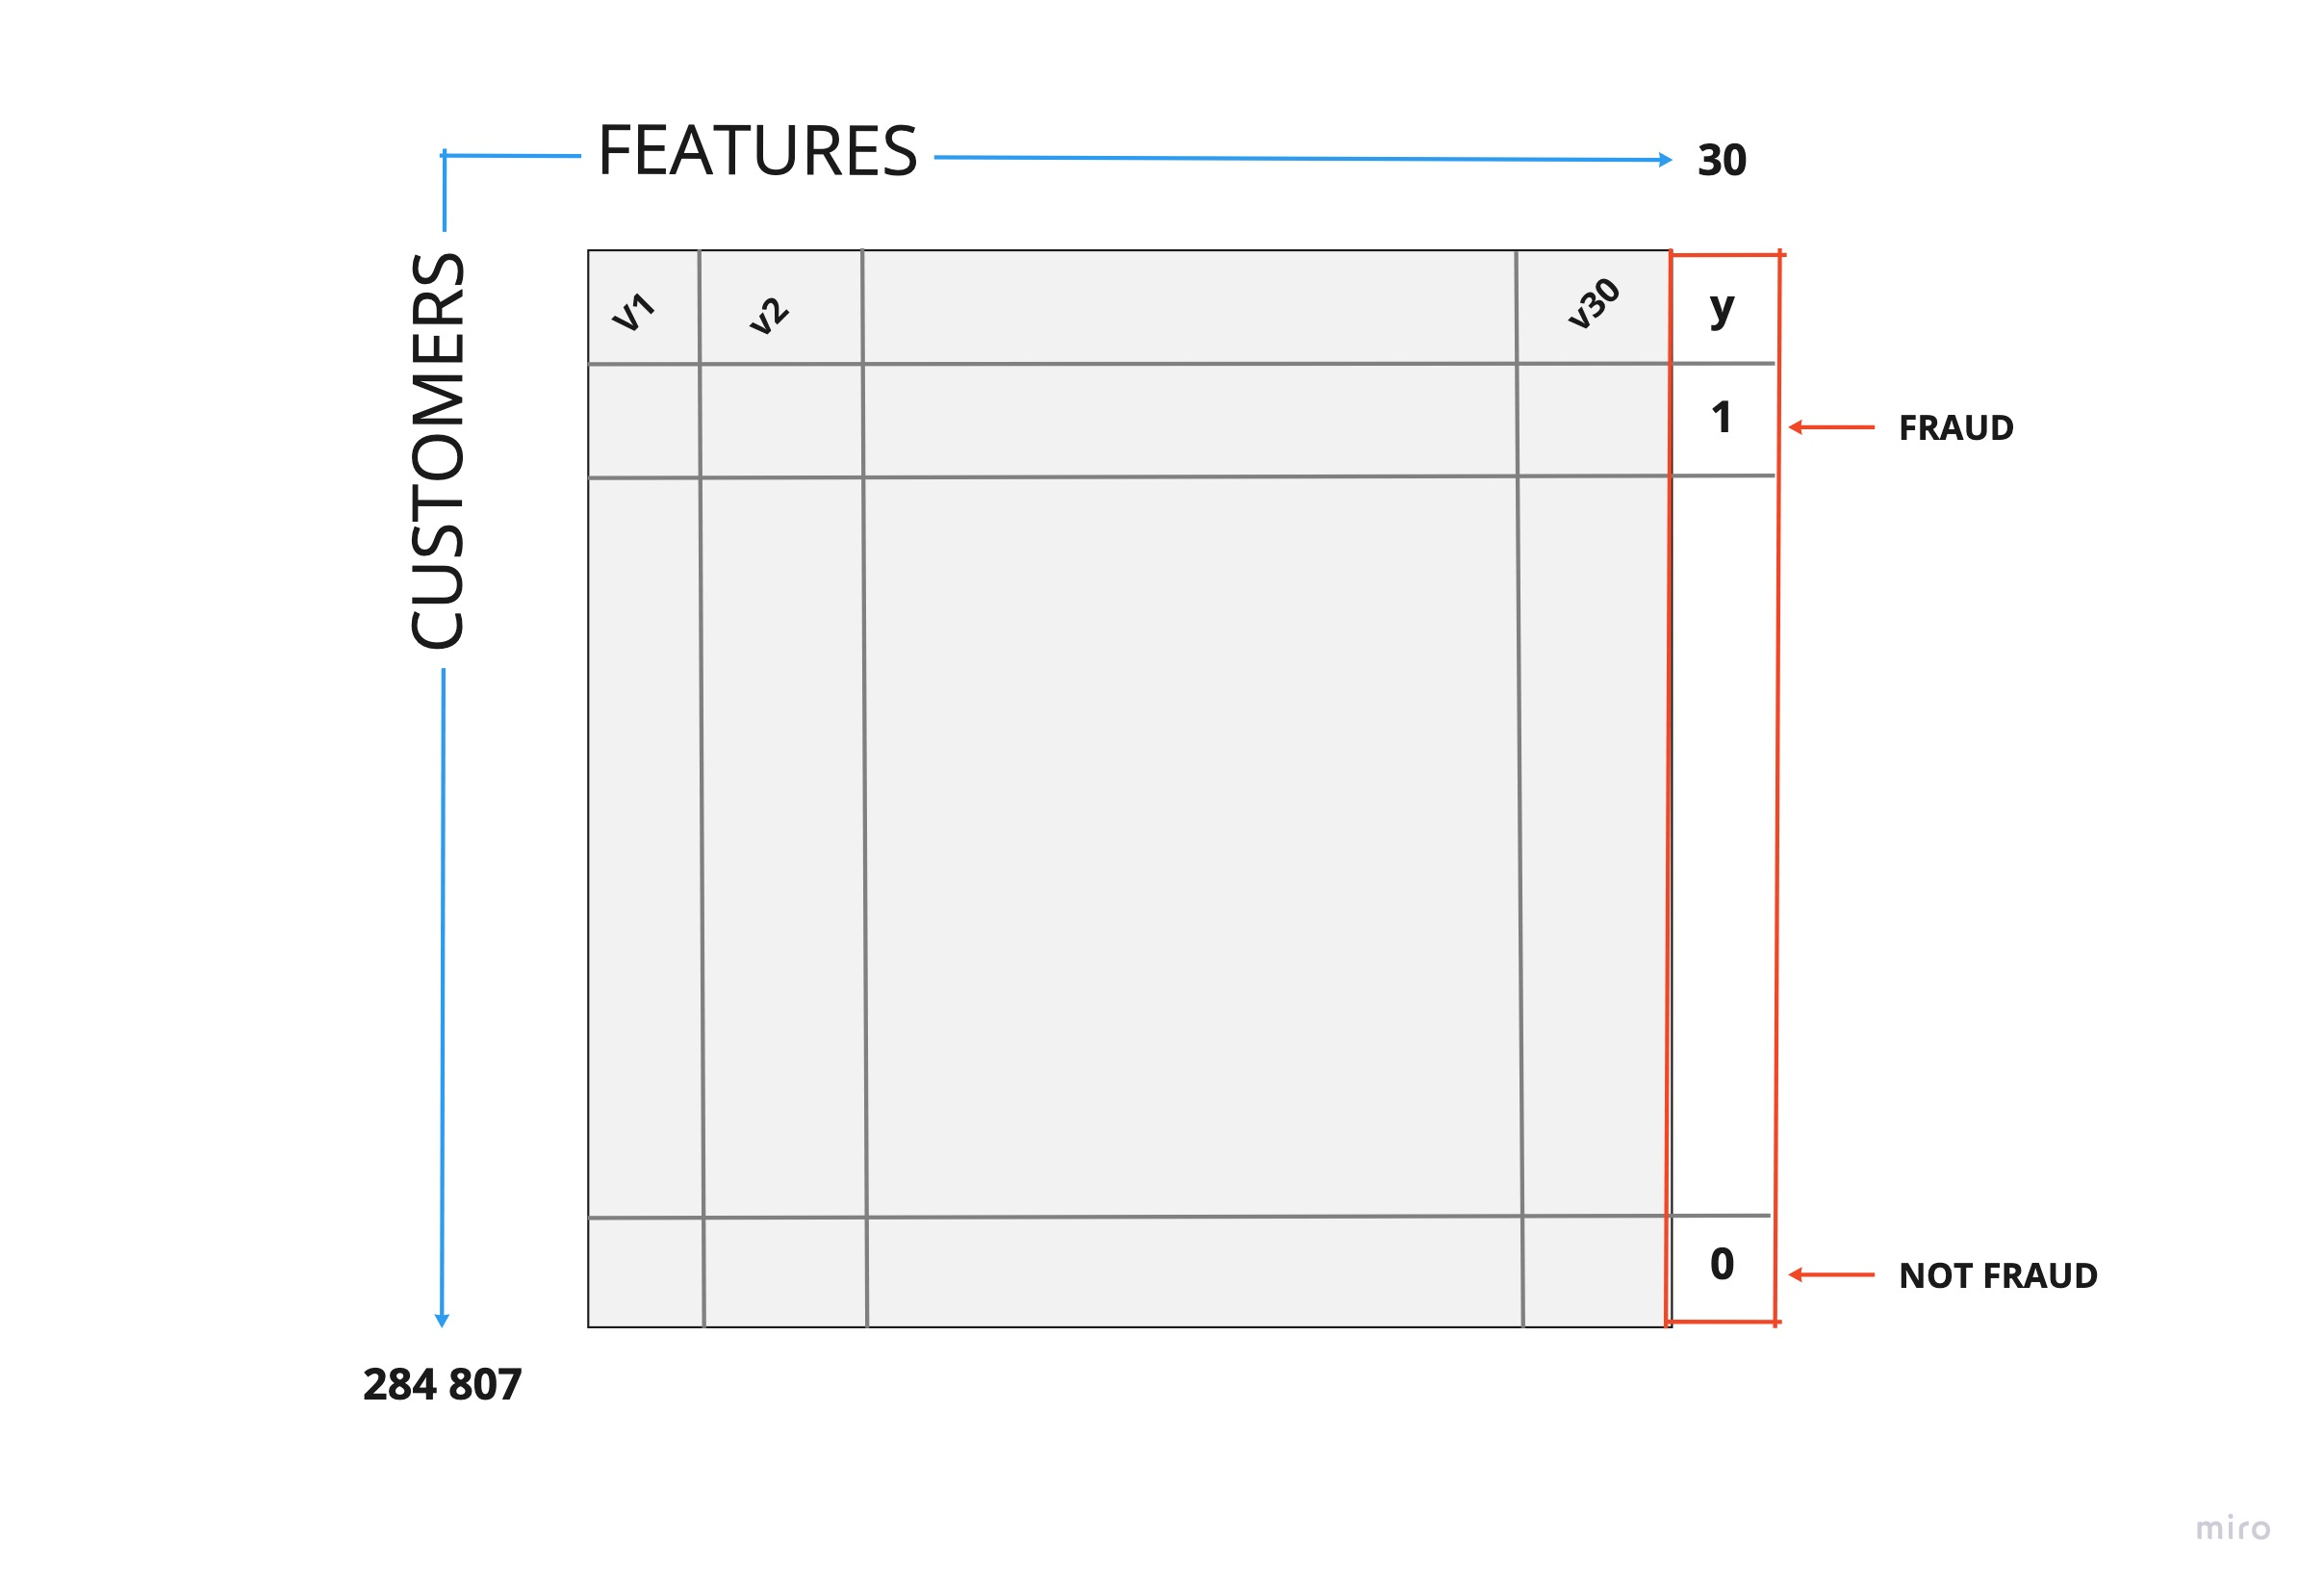
\includegraphics[width=10cm]{images/DATASET.jpg}
    \caption {The dataset high level overview.}
    \label{fig:ct_spine}
\end{figure}

It contains only numerical input variables which are the result of a PCA transformation. Unfortunately, due to confidentiality issues, we cannot provide the original features and more background information about the data. Features V1, V2, … V28 are the principal components obtained with PCA, the only features which have not been transformed with PCA are 'Time' and 'Amount'. Feature 'Time' contains the seconds elapsed between each transaction and the first transaction in the dataset. The feature 'Amount' is the transaction Amount, this feature can be used for example-dependant cost-senstive learning. Feature 'Class' is the response variable and it takes value 1 in case of fraud and 0 otherwise.

\section{Experiments}
We had validated the Neural Forest models experimentally (Independent Training  and Joint Training) and compared them with standard Random Forests and other competitors. 

\subsection{Machine Properties}
Within the experiments it was used macbook pro middle 2018 with Coffee Lake/8th generation: a 2.2GHz Core i7 processor with six cores and with intel turbo boost up to 4.1GHz.

\subsection{Results}
Table summarizes the results in terms of accuracy for the different models. The first important comment is that all Neural Forest models improve over the original Random Forest. Thus the Neural Forest are indeed more competitive than the original random forests which they were derived from. 
\begin{figure}[h]
    \centering 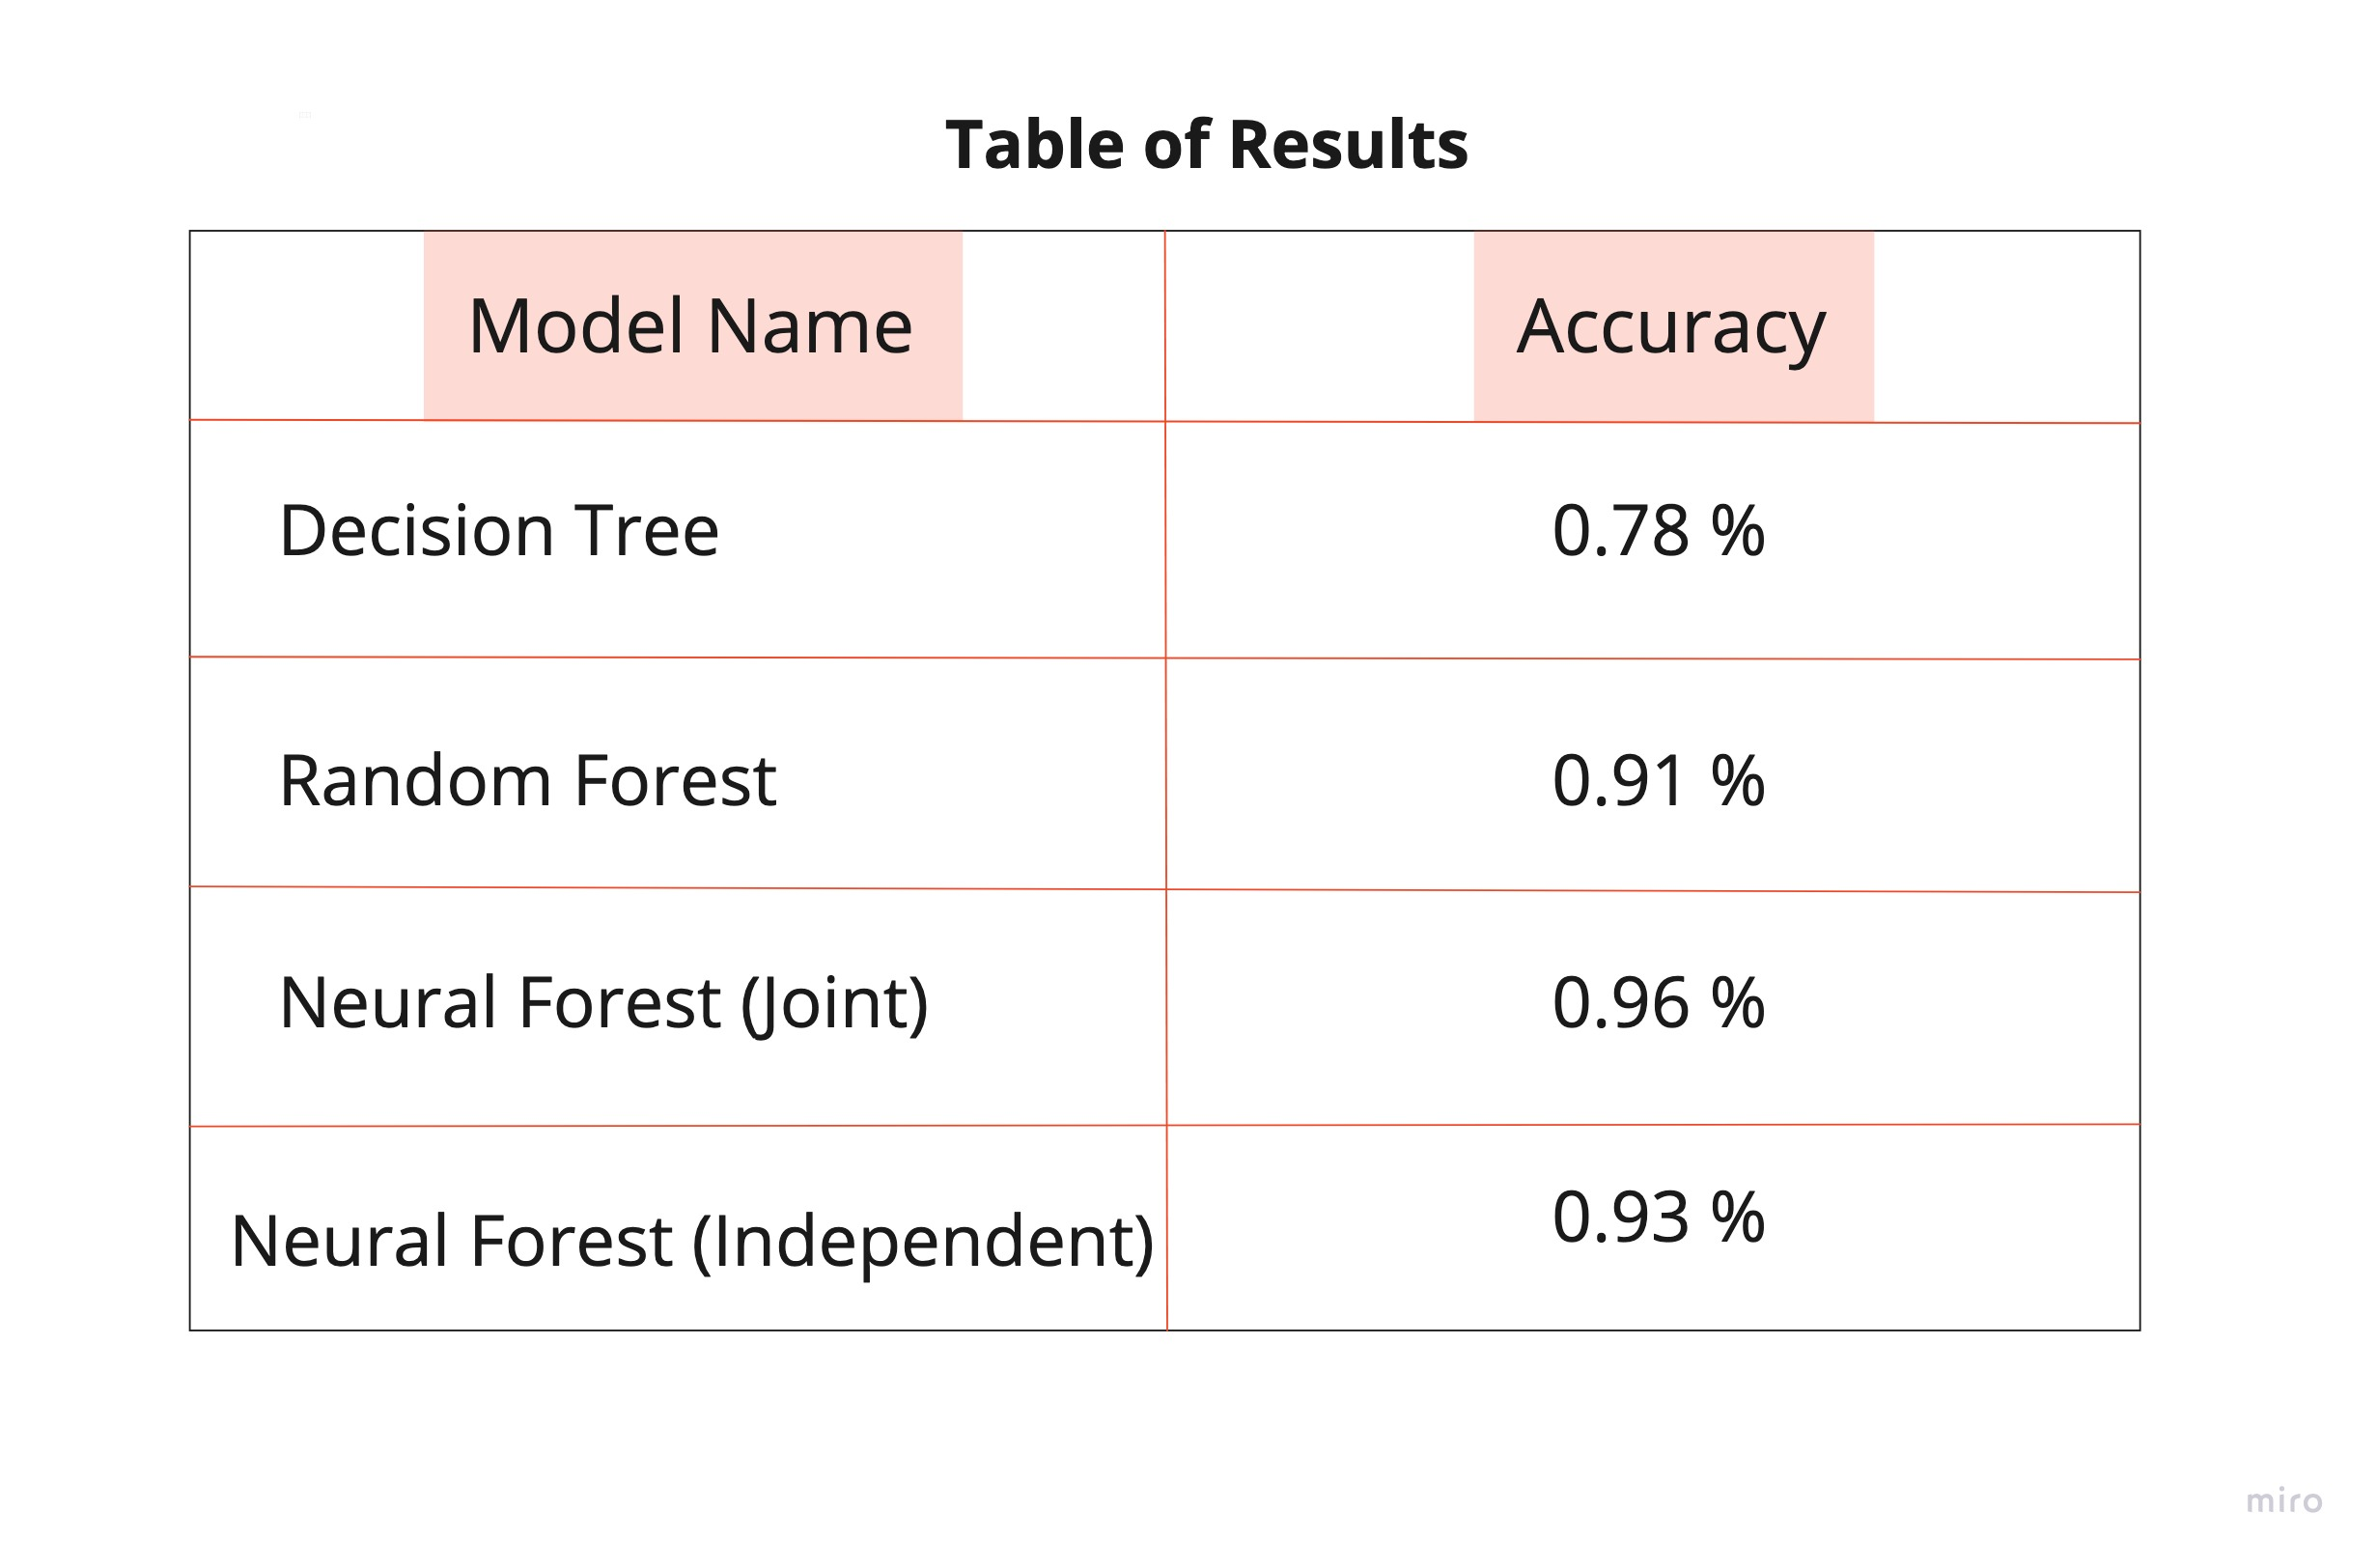
\includegraphics[width=10cm]{images/TableofResults.jpg}
    \caption {The table of results.}
    \label{fig:ct_spine}
\end{figure}

\section{Conclusion}
In this paper we have shown how to model and train stochastic, differential decision trees, usable as alternative classifiers for end-to-end learning in (deep) convolutional networks. Prevailing approaches for decision tree training typically operate in a greedy and local manner, making representation learning impossible. To overcome this problem, we introduced stochastic routing for decision trees, enabling split node parameter learning via backpropagation. Moreover, we showed how to populate leaf nodes with their optimal predictors, given the current state of the tree/underlying network.


\printbibliography

\end{document}










